\documentclass[12pt]{article}
\usepackage{amssymb,amsmath,latexsym}
\usepackage{graphicx}

% Page length commands go here in the preamble
\setlength{\oddsidemargin}{-0.25in}  % Left margin of 1 in + 0 in = 1 in
\setlength{\textwidth}{7in}  % Right margin of 8.5 in - 1 in - 6.5 in = 1 in
\setlength{\topmargin}{-.75in}  % Top margin of 2 in -0.75 in = 1 in
\setlength{\textheight}{9.2in}  % Lower margin of 11 in - 9 in - 1 in = 1 in

%\renewcommand{\baselinestretch}{1.5}  % 1.5 denotes double spacing. Changing it will change the spacing

\setlength{\parindent}{0in} 
\begin{document}
\title{CS 440 -- Intro to AI \\ Report 3: Heuristic Search}
\author{Skyler Malinowski (som12) \\ Andrew Dos Reis (ad1005)}
\date{December 6, 2017}
\maketitle

\newpage

\section{Part A}
% Show sample of interface
Our implementation makes use of a GUI and terminal to display relevant information. The GUI displays the map with color denoting what kind of cells they are and a path trace for the shortest path found. Whilest the terminal is used to display information regarding the cell that was clicked on. Of such information is the location of node \(n\), in programming notation, and the values corresponding to variables in \(f(n) = g(n) + h(n)\).

\section{Part B}
% (15 points)
\subsection{A*}
% Insert Example Solution with information
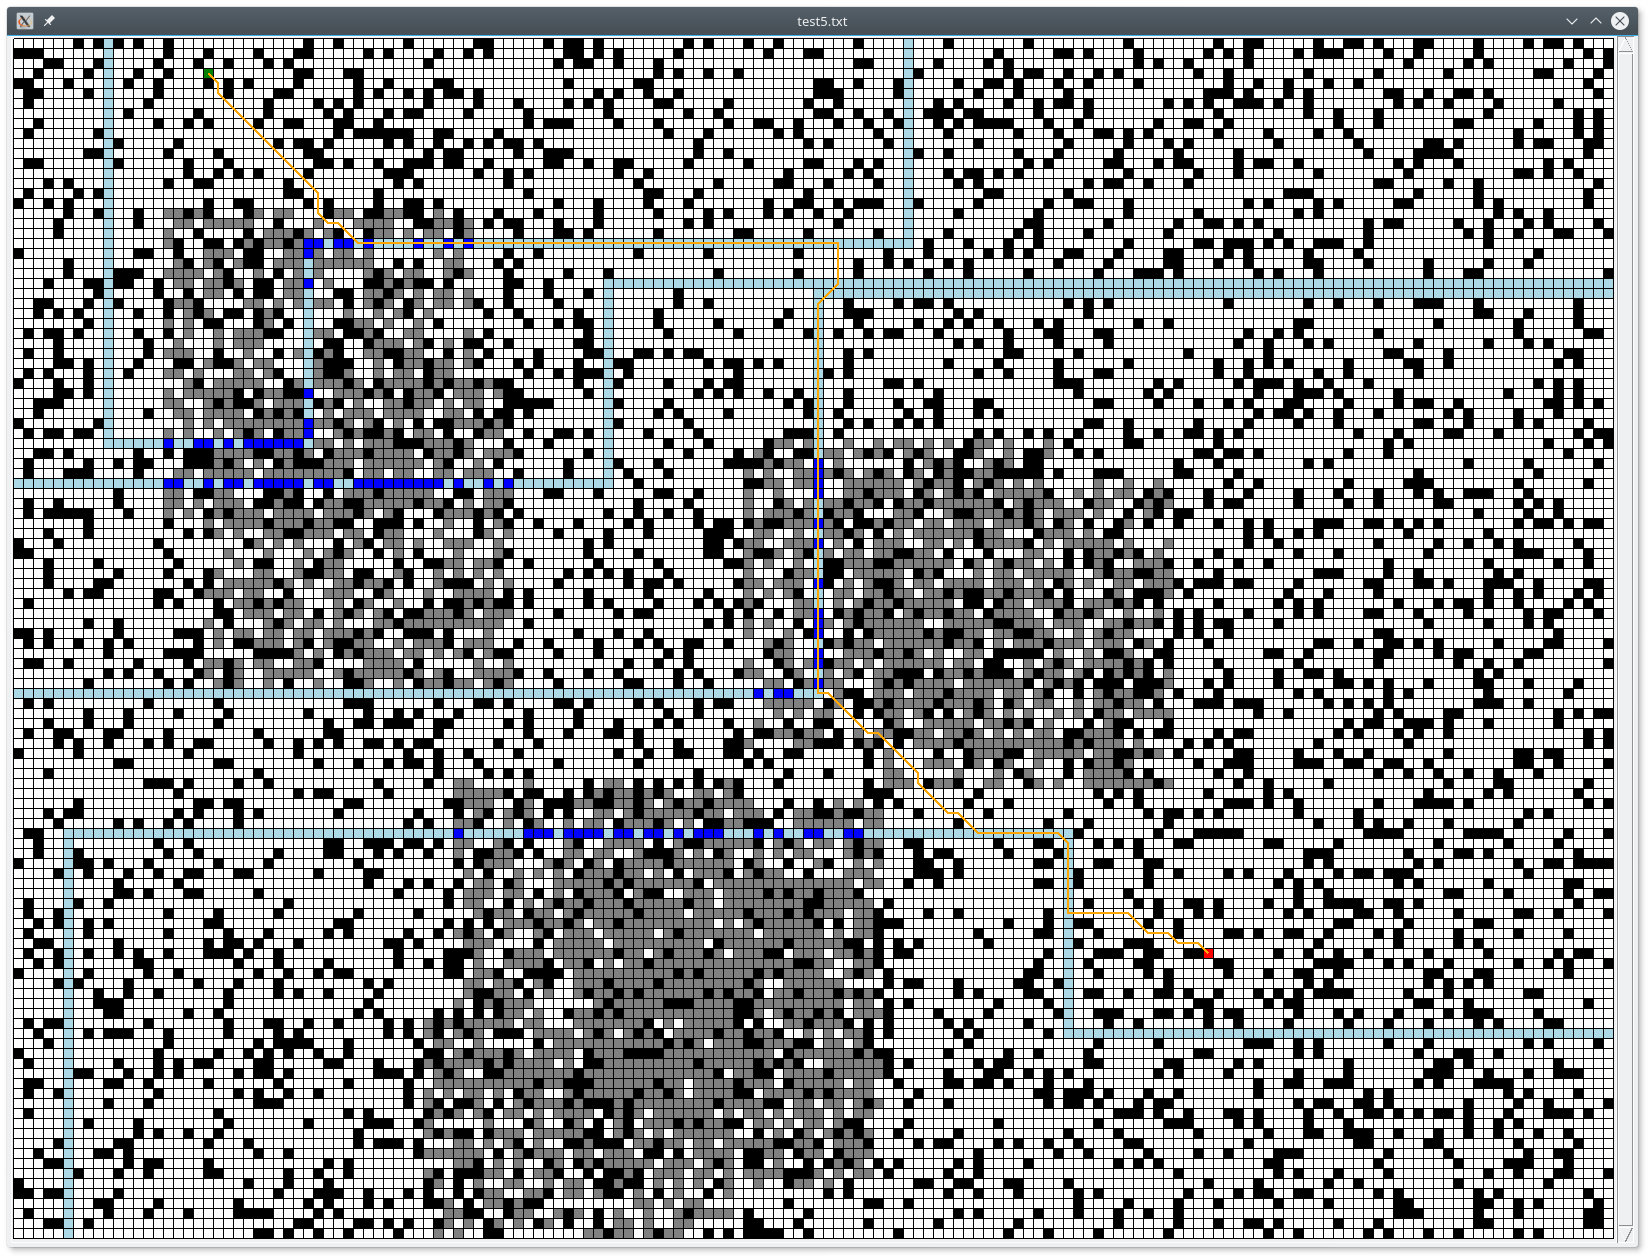
\includegraphics[scale=0.415]{aStar1.png}
\newline
Shortest Path Length: 99.27260094890539

\subsection{Weighted A*}
% Insert Example Solution with information
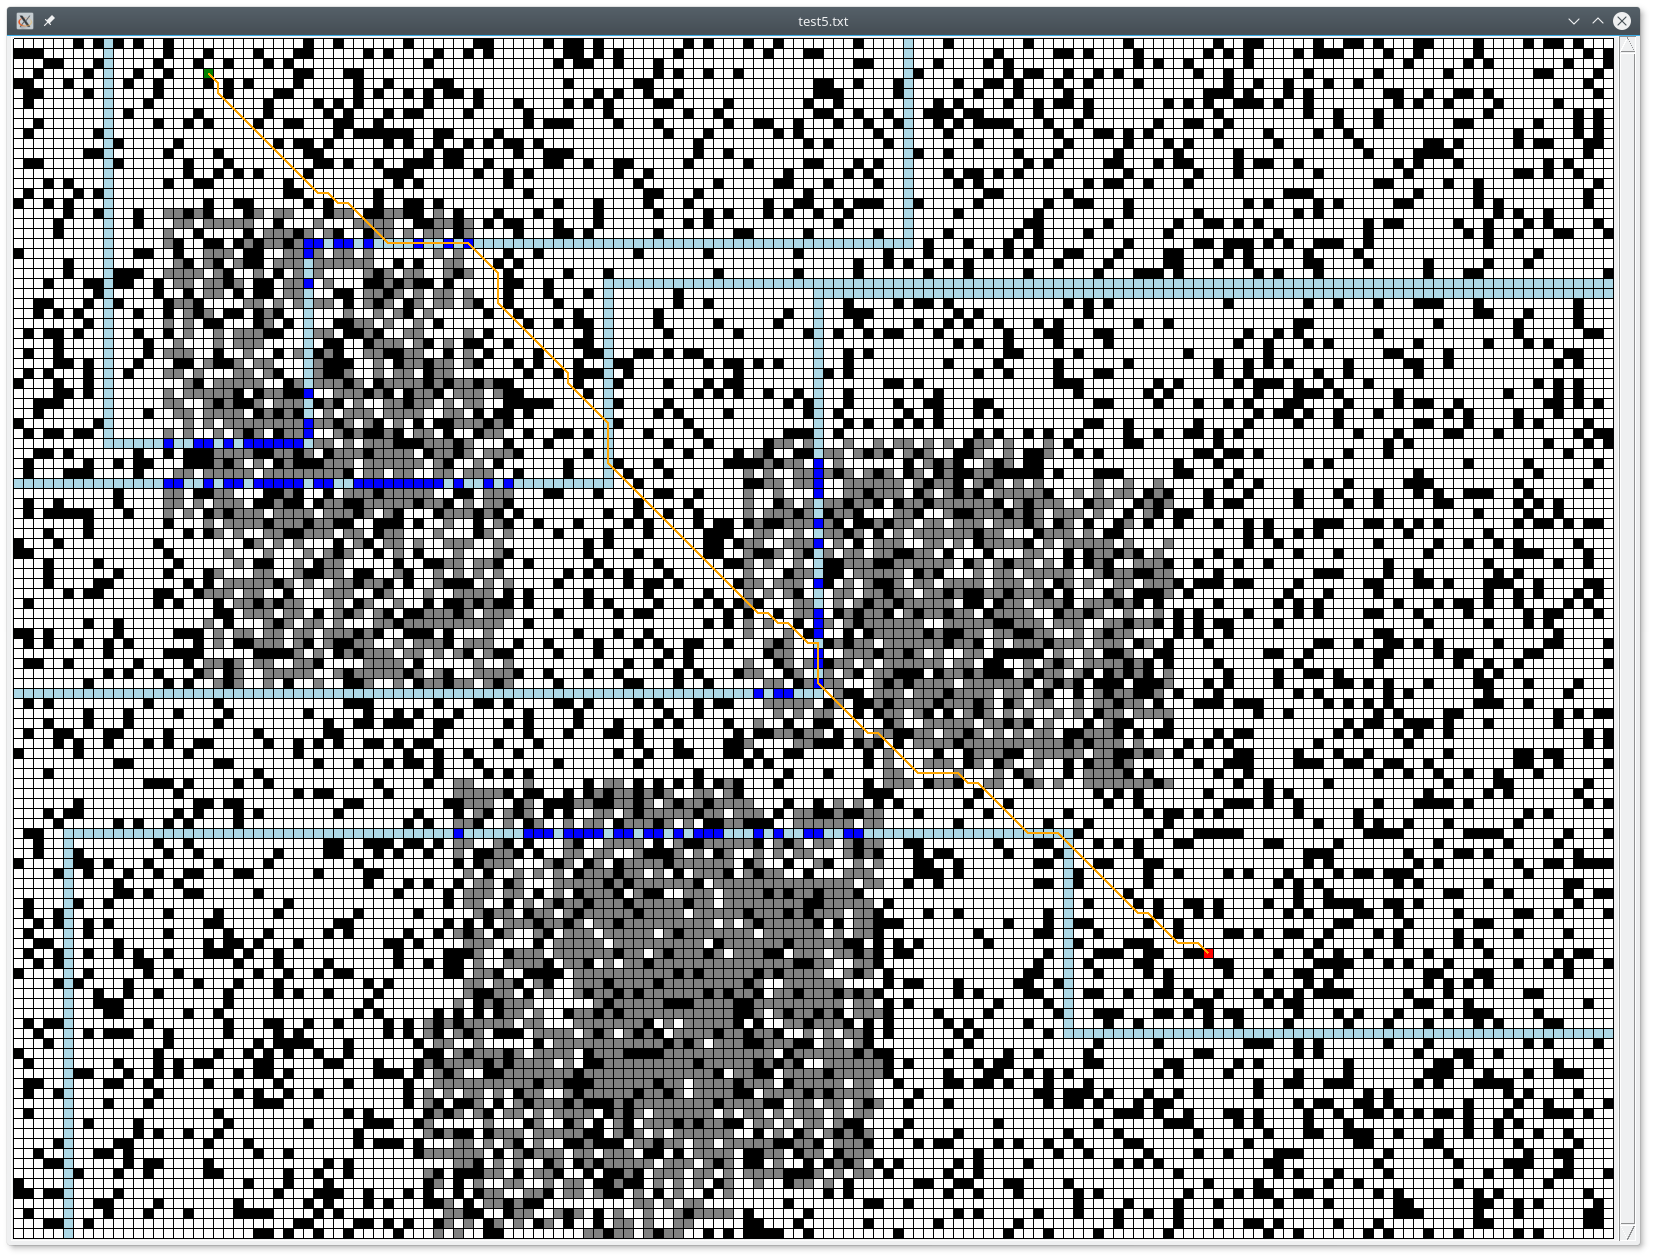
\includegraphics[scale=0.415]{W1_5_aStar1.png}
\newline
Shortest Path Length (\(w = 1.5\)): 138.07642481806775

\subsection{Uniform Cost Search}
% Insert Example Solution with information
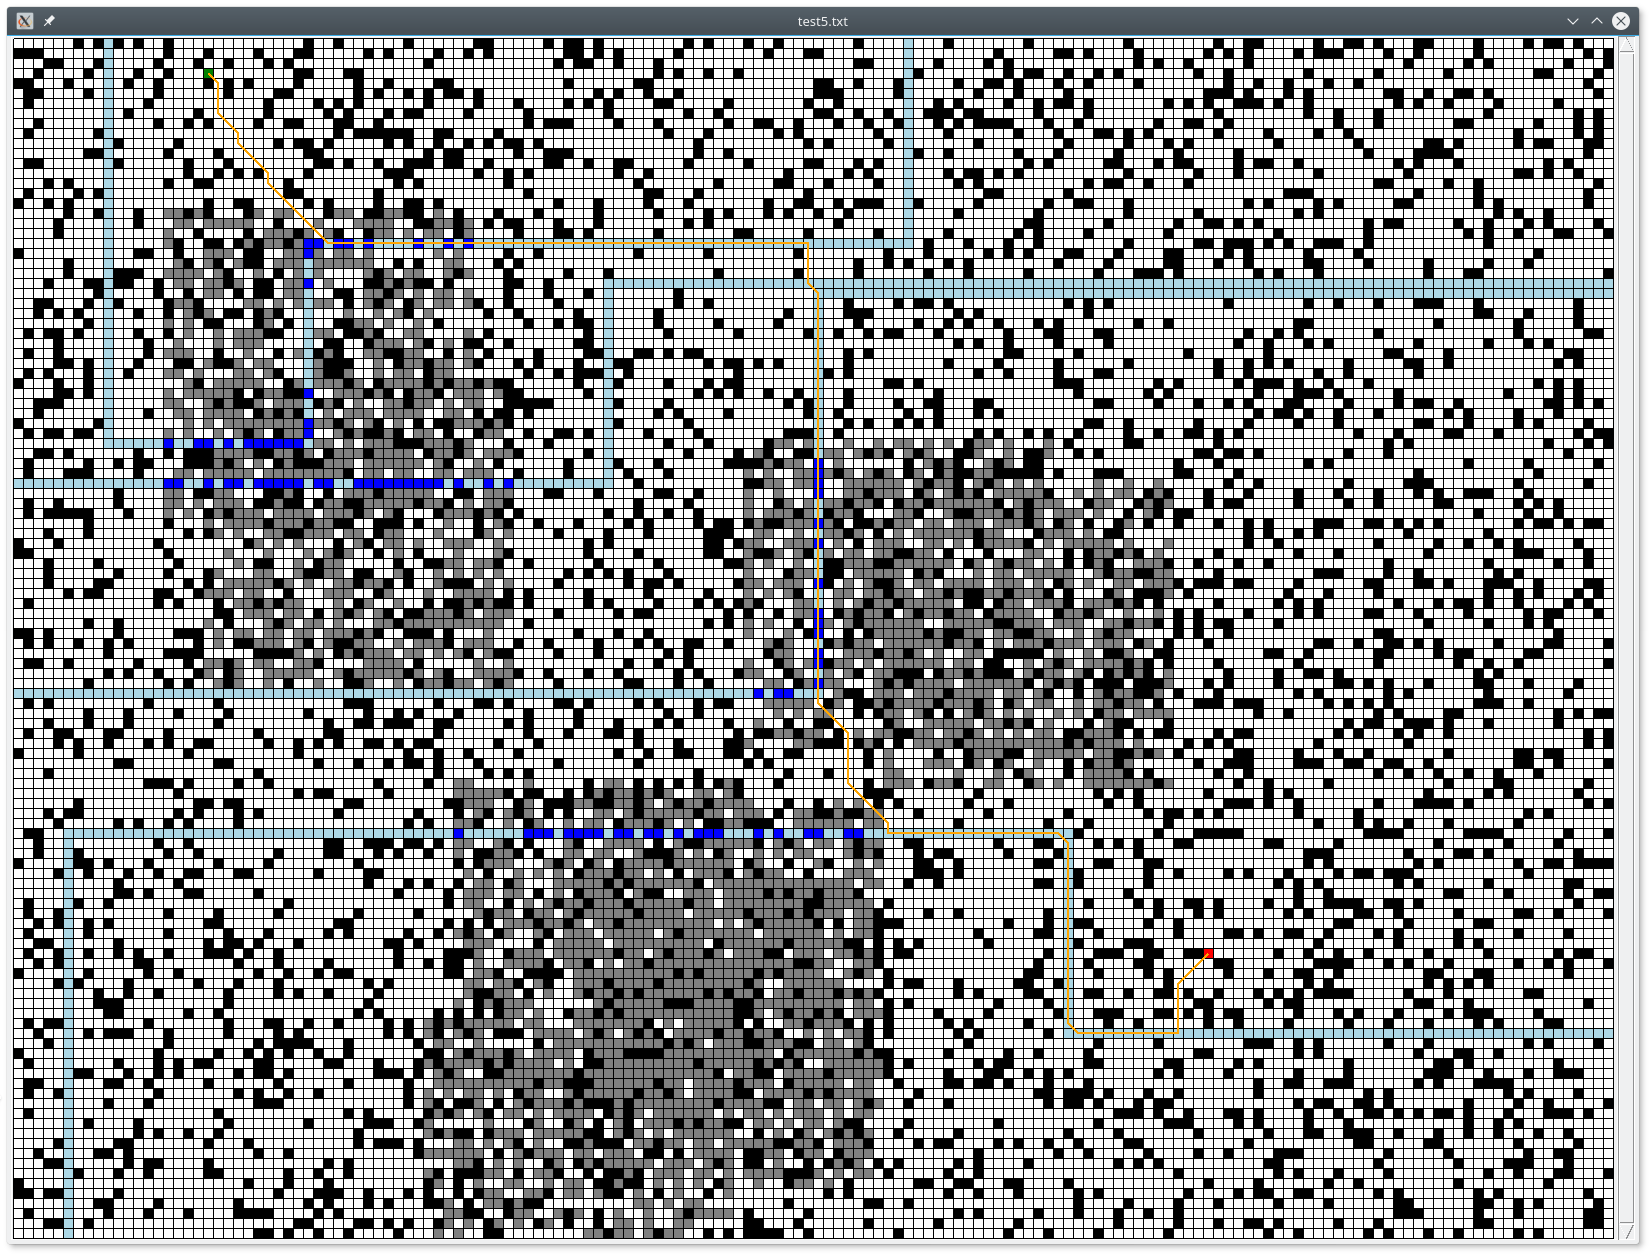
\includegraphics[scale=0.415]{Uniform1.png}
\newline
Shortest Path Length: 94.00178566873412

\section{Part C}
% Optimize your implementation of the above algorithms. Discuss your optimizations in your report. (10 points)
There were few points of optimizations made to our algorithms.
\begin{itemize}
  \item A prioity queue on the open list with \(f(n)\) being the priority factor. This is to ensure that the algorithm is not uselessly expanding nodes that with higher probability will not lead to optimal solution. To do this we implemented the priority queue for the open list as a Binary Heap which naturally orders its contents in ascending order so that the first item popped off of the queue is the largest in value. This saves time and memory by not having to search through the open list to find the largest \(f(n)\) value.
  \item Making sure the heuristic is admissible. In an effort to ensure it never overestimates, the heuristic is modified by the best case movement cost for the world in question. Also the base heuristicmust have the right amount of degrees of freedom. Because our agent can move in eight directions, the heuristic chosen must also have that as its minimum degrees of freedom to have a better solutions arrived at. If either is breached, so is admissibility.
  \item Making a modular implementation of A*. To achieve such, Python imheritance was leveraged, weights were inserted, and functions were used to ensure a scalable and modular implementation.
\end{itemize}

\section{Part D}
% Propose different types of heuristics for the considered problem and discuss them in your report. In particular:
% • Propose the best admissible/consistent heuristic that you can come up with in this grid world.
% • Propose at least four other heuristics, which can be inadmissible but still useful for this problem and justify your choices.
% Remember that good heuristics can effectively guide the exploration process of a search algorithm towards finding a good solution fast and they are computationally inexpensive to compute. (10 points)
These are the Heuristics we implemented, where Modified indicates that it was multiplied by the lowest terrain travel cost coefficient and Raw means it is the standard implementation of that Heuristic without a coefficient.
\subsection{Modified Euclidean Distance}
 \[ h = (0.25) * \sqrt{ (x_{current} - x_{goal})^2 + (y_{current} - y_{goal})^2}\]
\newline
 Admissible because it underestimates the distance to the goal by assuming that it will be traveling on river tiles the entire path and because it accounts for full freedom of movement for our agent.
\subsection{Modified Chebyshev Distance}
  \[ h = (0.25) * \max( | x_{current} - x_{goal} |, | y_{current} - y_{goal} | )\]
\newline
Admissible because it underestimates the distance to the goal by assuming that it will be traveling on river tiles the entire path and because it accounts for full freedom of movement for our agent.
\subsection{Modified Manhattan Distance}
\[ h = (0.25) * ( | x_{current} - x_{goal} | + | y_{current} - y_{goal} | )\]
\newline
Inadmissible because while it underestimates the distance to the goal by assuming that it will be traveling on river tiles the entire path it does not account for the full freedom of movement our agent has in our world.
\subsection{Raw Chebyshev Distance}
 \[ h = \max( | x_{current} - x_{goal} |, | y_{current} - y_{goal} | )\]
\newline
Inadmissible because it does not underestimate the distance to the goal even though it does account for the full freedom of movement of our agent.
\subsection{Raw Manhattan Distance}
\[ h =  ( | x_{current} - x_{goal} | + | y_{current} - y_{goal} | )\] 
Inadmissible because it does not underestimate the distance to the goal and it does not account for the full freedom of movement of our agent.

\section{Part E}
% Perform an experimental evaluation on the 50 benchmarks using the three algorithms that you have implemented for the 5 different heuristics that you have considered. For Weighted A∗ you should try at least two w values, e.g., 1.25 and 2 (feel free to experiment). Compare the various solutions in terms of average run-time, average resulting path lengths as a function of the optimum length, average number of nodes expanded and memory requirements (average over all 50 benchmarks). In your report, provide your experimental results. (15 points)
\subsection{Table of Averages -- }
\begin{tabular}{|c|c|c|c|c|}
\hline
	Heuristic & Average Path Cost & Nodes Expanded & Nodes Considered & Elapsed Time\\
\hline
	Uniform Cost & 104.26106823928 & 15206.9583333333 & 15205.9583333333 & 134.628174041667\\
\hline
	Custom Euclidean Distance & 104.247383775749 & 12659.7916666667 & 12658.7916666667 &102.849767291667 \\
\hline
	Custom Euclidean Distance 1.5 & 104.247383775749 & 11037.5416666667 & 11036.5416666667 & 81.3740608750001\\
\hline
	Custom Euclidean Distance 2.0 & 104.541599741667 & 12231.5416666667 & 12230.5416666667 & 122.428055166667\\
\hline
	Raw Manhattan & 129.202789733504 & 3030.16666666667 & 3029.16666666667 & 9.72364704166663\\
\hline
	Raw Manhattan 1.5 & 159.577792698078 & 1 & 6.3\\
\hline
	Raw Manhattan 2.0 &  & 1 & 6.3\\
\hline
	Raw Chebyshev & & 2501.4 & 3277.4\\
\hline
	Raw Chebyshev 1.5&  & 2501.4 & 3277.4\\
\hline
	Raw Chebyshev 2.0& & 2501.4 & 3277.4\\
\hline
	Modified Manhattan &  & 1251.4 & 1504.1\\
\hline
	Modified Manhattan 1.5&  & 1251.4 & 1504.1\\
\hline
	Modified Manhattan 2.0&  & 1251.4 & 1504.1\\
\hline
	Modified Chebyshev &  & 3816.1 & 4185.4\\
\hline
	Modified Chebyshev 1.5&  & 3816.1 & 4185.4\\
\hline
	Modified Chebyshev 2.0&  & 3816.1 & 4185.4\\

\hline
\end{tabular}



\section{Part F}
% Explain your results and discuss in detail your observations regarding the relative performance of the different methods. What impact do you perceive that different heuristic functions have on the behavior of the algorithms and why? What is the relative performance of the different algorithms and why? (10 points)
The above table was generated by taking the average of a series of 50 benchmark tests made up of 5 maps run 10 times with different start and goal positions each time. The result is data to describe on average the difference between each Heuristic and version of A Star through their path costs, nodes expanded count, nodes considered count, and time elapsed.
\newline
\newline
The distinction between the different Heuristics largely came in the Nodes Expanded and Nodes Considered data. For admissible Heuristics (Uniform Cost, Modified Euclidean, and Modified Chebyshev) the standard un-weighted path cost average were identical across the board proving their property of never overestimating the distance. For each of the admissible Heuristics the weighted version at 1.5 nominally reduced the Nodes expanded and Nodes considered count. Interestingly the further weighted 2.0 version either negates some of that decrease or actually increases those metrics while also making it not admissible for some worlds, leading to a very minor increase in the average path cost for all of the 2.0 weighted admissible heuristics. 
\newline
\newline
Between the Admissible Heuristics it is clear that Uniform Cost is the least efficient having a considerably larger average Node Expanded Count then the other two. Modified Euclidean and Modified Chebyshev are very close in their resource use but its clear from the average that Modified Euclidean uses just a little bit less memory from the Nodes Expanded and Nodes Considered averages.
\newline
\newline
The Inadmissible Heuristics (Raw Manhattan, Raw Chebyshev, and Modified Manhattan) clearly show their usefulness by being considerably faster to run then the admissible ones on average. Add on top of that their considerably lower overhead costs from much lower Nodes Expanded and Nodes Considered counts and its clear to see why it was important to experiment with both Admissible and Inadmissible Heuristics. The Inadmissible heuristics, as their name implied fell short of the actual minimum path costs set by the Admissible heuristics but not to a huge degree, the degree by which they ran faster and lighter then the Admissible heuristics far overshadowed the degree by which their path costs increased. Unlike with the Admissible Heuristics though, the 1.5 weighting and 2.0 weighting both considerably further reduce the Nodes Expanded and Nodes Considered.
\newline
\newline
As for the order of efficiency for the Inadmissible heuristics it is clear by the data that when unweighted the Raw Manhattan heuristic is the most efficient in terms of Nodes expanded and Nodes Considered, followed by Custom manhattan and then Raw Chebyshev. 

\section{Part G}
% Implement the Sequential Heuristic A∗. Use an admissible heuristic for the anchor search. Use 4 other heuristics, admissible or inadmissible ones, for the remaining search processes. You should try at least two w1 and two w2 values, e.g., 1.25 and 2 (feel free to experiment). Make choices so as to optimize the performance of the algorithm, i.e., aim for solutions that compute as high-quality solutions and as fast as possible.
% Perform an experimental evaluation over the 50 benchmarks you have considered above. In particular, compare the A∗ approach with the admissible heuristic against the Sequential Heuristic version, which utilizes all the heuristics you have considered. Compare the various solutions in terms of average runtime, average resulting path lengths as a function of the optimum length, average number of nodes expanded and memory requirements (average over all 50 benchmarks). In your report, provide your experimental results. (15 points)
The admissable heuristic chosen for the anchor search was a modified Euclidean. The other heuristics chosen were as disccussed in Part C. As for weights, our weight sets chosen were \([w_1,w_2] = [1.25,2],[2,1.25]\).

\subsection{Table of Averages -- Weights = [1.25, 2]}
\begin{tabular}{|c|c|c|c|c|}
\hline
	Heuristic & Weights & Nodes Expanded & Nodes Considered\\
\hline
	Modified Euclidean & [1.25, 2] & 7695.7 & 8191.5\\
\hline
	Raw Manhattan & [1.25, 2] & 1 & 6.3\\
\hline
	Raw Chebyshev & [1.25, 2] & 2501.4 & 3277.4\\
\hline
	Modified Manhattan & [1.25, 2] & 1251.4 & 1504.1\\
\hline
	Modified Chebyshev & [1.25, 2] & 3816.1 & 4185.4\\
\hline
\end{tabular}
\newline
Average Elapsed Time = 142.85

\subsection{Table of Averages -- Weights = [2, 1.25]}
\begin{tabular}{|c|c|c|c|c|}
\hline
	Heuristic & Weights & Nodes Expanded & Nodes Considered\\
\hline
	Modified Euclidean & [2, 1.25] & 7622.3 & 8247.6\\
\hline
	Raw Manhattan & [2, 1.25] & 1 & 6.3\\
\hline
	Raw Chebyshev & [2, 1.25] & 1 & 6.3\\
\hline
	Modified Manhattan & [2, 1.25] & 1 & 6.3\\
\hline
	Modified Chebyshev & [2, 1.25] & 2541.4 & 2860.4\\
\hline
\end{tabular}
\newline
Average Elapsed Time = 127.055

\section{Part H}
% Describe in your report why your implementation is efficient. Explain your results and discuss in detail your observations regarding the relative performance of the methods. Discuss the relationship with your experiments for section e. What is the relative performance of the different algorithm in terms of computation time and solution quality and why? (10 points)
What makes Sequential A* efficient is the ability to sequentially test multiple heuristics to arrive at the best. By best, I mean the heuristic that can beat out the anchor heuristic implying that the winner is admissable, consistant, and more efficient than the anchor heuristic.
\newline
\newline
From the table, Raw Manhattan Distance is the worst (as to be expected). Surprisingly, Modified Manhattan Distance got further than it's Raw equivalent under certain weights. Good but still not great. Unsurprisingly, Modified Euclidean Distance was more often than not expanded to full over the other heuristics; Modified Chebyshev Distance come in second, albeit by a huge margin. We thought that Modified Chebyshev Distance would have scored better than Modified Euclidean Distance because the it calculates distance in the same way that the agent can move -- eight degrees of freedoms.
\newline
\newline
% Talk about Part E in context of Part H -- relationship and performance.



\end{document}